\documentclass[10pt]{article}
\usepackage[margin=0.60in]{geometry}
\usepackage{booktabs,enumitem,fancyhdr,graphicx,listings,tabularx,titlesec,xcolor}
\usepackage[hidelinks]{hyperref}
\graphicspath{{docs/lessons/assets/}{../assets/}}
\hypersetup{
 pdftitle={ADK Lesson 059: Recorded MAX7219 Presentation},
 pdfauthor={Kevin Shanahan},
 pdfsubject={Deterministic MAX7219 register intent, orientation transforms, copied transport receipts, and partial-write fault provenance},
 pdflang={en-US}}
\pagestyle{fancy}\fancyhf{}
\lhead{\textsc{ADK Lesson 059}}\rhead{Recorded MAX7219 Presentation}
\cfoot{\thepage}\setlength{\headheight}{14pt}
\setlength{\parindent}{0pt}\setlength{\parskip}{3pt}
\setlist{nosep,leftmargin=1.45em}
\titleformat{\section}{\Large\bfseries}{\thesection}{0.5em}{}
\newcommand{\lessonbox}[1]{\begin{center}\fbox{\parbox{0.92\linewidth}{#1}}\end{center}}
\newcommand{\blankline}{\rule{0.76in}{0.4pt}}
\newcommand{\longblank}{\rule{1.28in}{0.4pt}}
\lstset{
 basicstyle=\ttfamily\footnotesize,
 columns=fullflexible,
 breaklines=true,
 frame=single,
 rulecolor=\color{black},
 showstringspaces=false}

\begin{document}
\small
\begin{center}
 {\Huge\bfseries Recorded MAX7219 Presentation}\\[3pt]
 {\Large Prove every register intent without pretending pixels changed}\\[7pt]
 \fbox{\textbf{E0 COPIED POLICY REPLAY --- ZERO DISPLAY HARDWARE}}
\end{center}
\begin{tabularx}{\linewidth}{@{}>{\bfseries}l X >{\bfseries}l X@{}}
Lesson & 059 --- component & Time & 120--180 minutes\\
Prerequisite & Lesson 058 transaction evidence & Board & compile-only Mega replay\\
Capacity & fixed 8-by-8 logical frame & Observation & command and receipt result cells\\
\end{tabularx}

\lessonbox{\textbf{Responsibility.}
\texttt{Max7219PresentationPolicy} transforms one copied 8-by-8 logical frame
into a bounded sequence of MAX7219 register commands. It owns policy state and
fault provenance. It owns no SPI bus, chip-select pin, module, resistor,
display, supply, clock, retry loop, or powered circuit.}

\section{Begin dark, then earn normal operation}
The MAX7219 is a write-only presentation endpoint in this lesson. A controller
can submit bytes, but it cannot read pixels back. Lesson 059 therefore starts
with a narrower claim: the policy can prove which command it requested and
which copied transport receipt it accepted.

Initialization keeps the logical device dark while it requests configuration.
The ordered sequence disables display test, disables decode mode, selects all
eight rows, sets bounded intensity, clears rows one through eight, and requests
normal operation last. Display test is not used as learner self-test evidence.

\begin{center}
% ADK visual: pencil
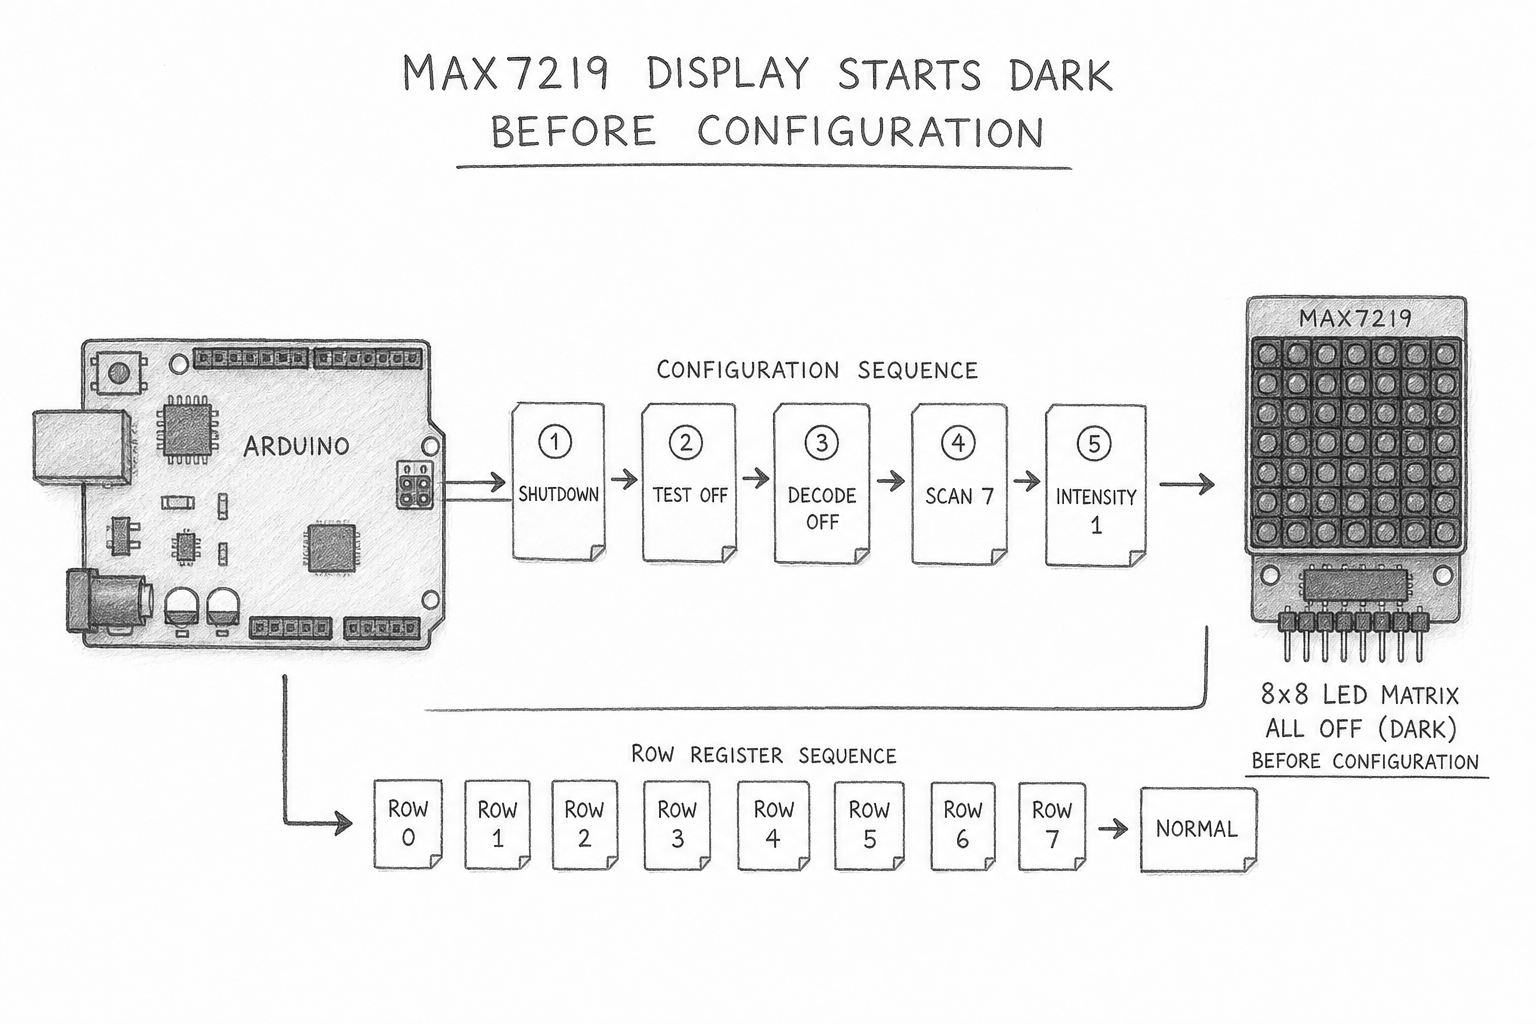
\includegraphics[width=0.95\linewidth,height=2.15in,keepaspectratio]
 {059-dark-start-pencil.png}

\small\textit{Alternative text: a pencil storyboard begins with a dark
eight-by-eight matrix, passes through configuration and eight cleared rows,
then reaches normal operation only after the final accepted receipt.}
\end{center}

Predict why ``normal operation last'' matters:
\begin{enumerate}
 \item If row clearing happened after normal operation, what stale pattern
 might briefly be presented? \longblank
 \item Which copied evidence can prove the request order? \longblank
 \item Which physical fact remains unknown at E0? \longblank
\end{enumerate}

\section{Separate a logical frame from wire orientation}
The independent frame generator owns eight logical row bytes. Logical row zero
is the top row, and bit seven is the leftmost pixel before transformation.
Orientation is fixed at initialization as \texttt{Identity},
\texttt{Rotate90}, \texttt{Rotate180}, or \texttt{Rotate270}. This makes a
module-specific rotation explicit instead of silently editing artwork.

\begin{center}
% ADK visual: pencil
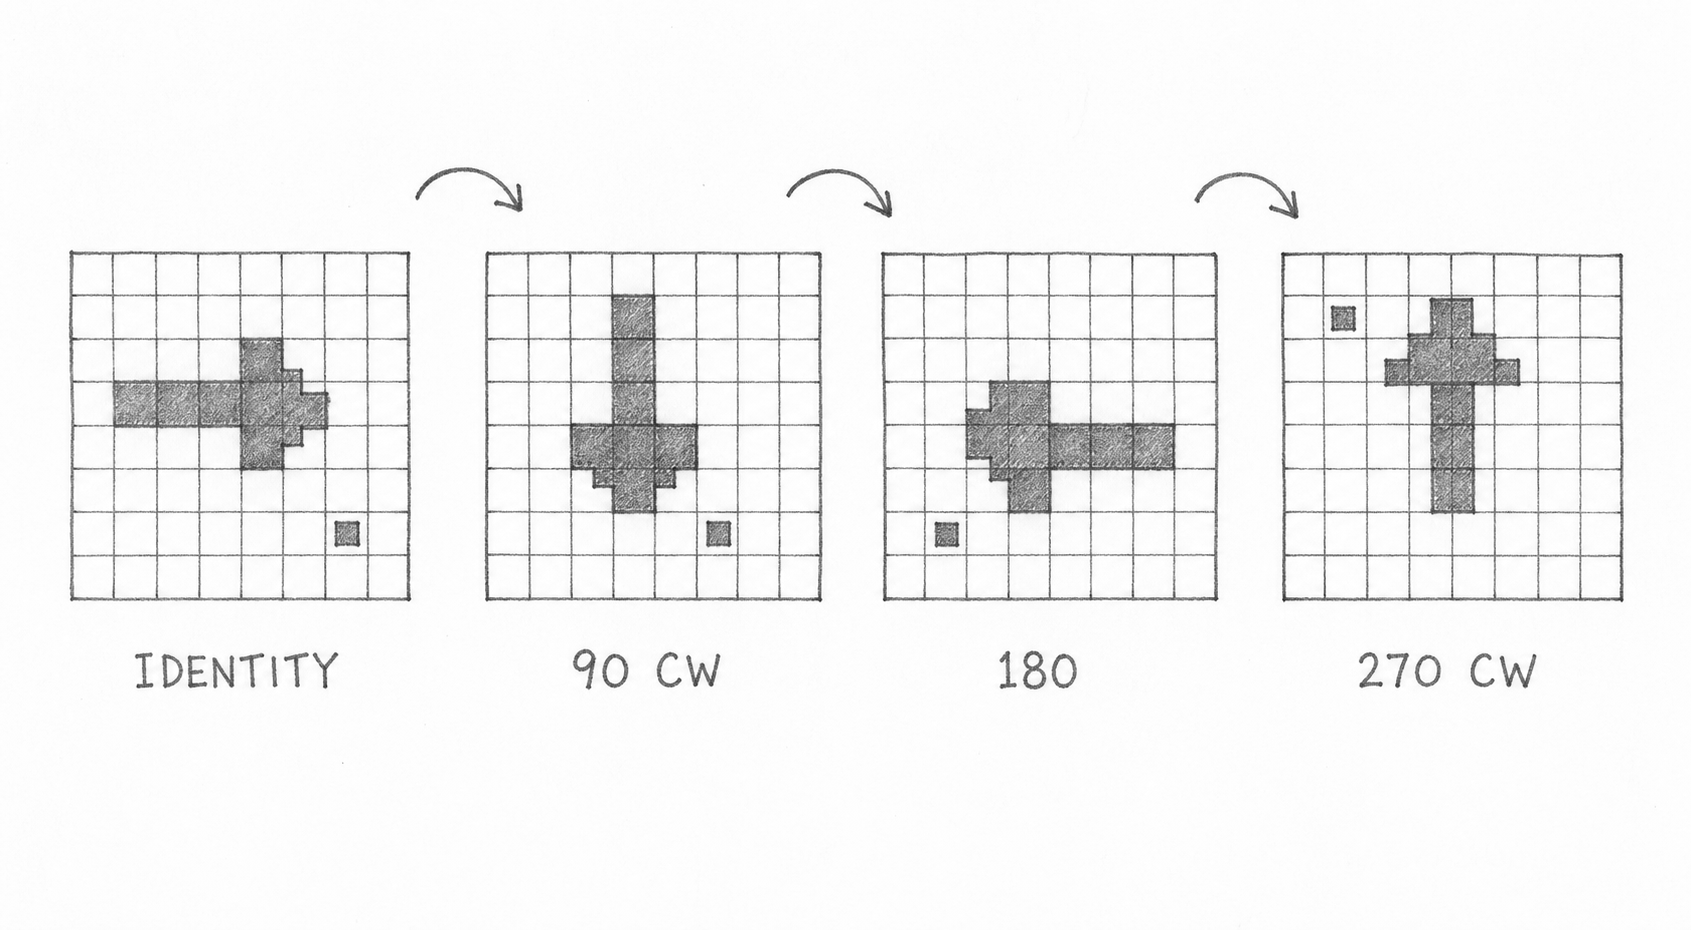
\includegraphics[width=0.94\linewidth,height=2.05in,keepaspectratio]
 {059-orientation-pencil.png}

\small\textit{Alternative text: four hand-drawn eight-by-eight grids show one
asymmetric arrow transformed through identity and rotations of 90, 180, and
270 degrees; a separate corner marker makes the clockwise movement visible.}
\end{center}

\begin{tabularx}{\linewidth}{@{}l X X@{}}
\toprule
Orientation & Predict the logical top-left pixel & Check\\
\midrule
\texttt{Identity} & remains at physical top left & transformed row 0, bit 7\\
\texttt{Rotate90} & moves to physical top right & expected row and bit\\
\texttt{Rotate180} & moves to physical bottom right & expected row and bit\\
\texttt{Rotate270} & moves to physical bottom left & expected row and bit\\
\bottomrule
\end{tabularx}

Use asymmetric test art. A filled square can look correct after the wrong
rotation and therefore proves very little.

\section{Read one register envelope}
Every published command is a copied value. It carries the owner token,
lifecycle generation, configuration revision, presentation generation,
operation index, register-address byte, and data byte. The intended MAX7219
transfer is exactly 16 bits, address first and data second, MSB first.

\begin{center}
% ADK visual: pencil
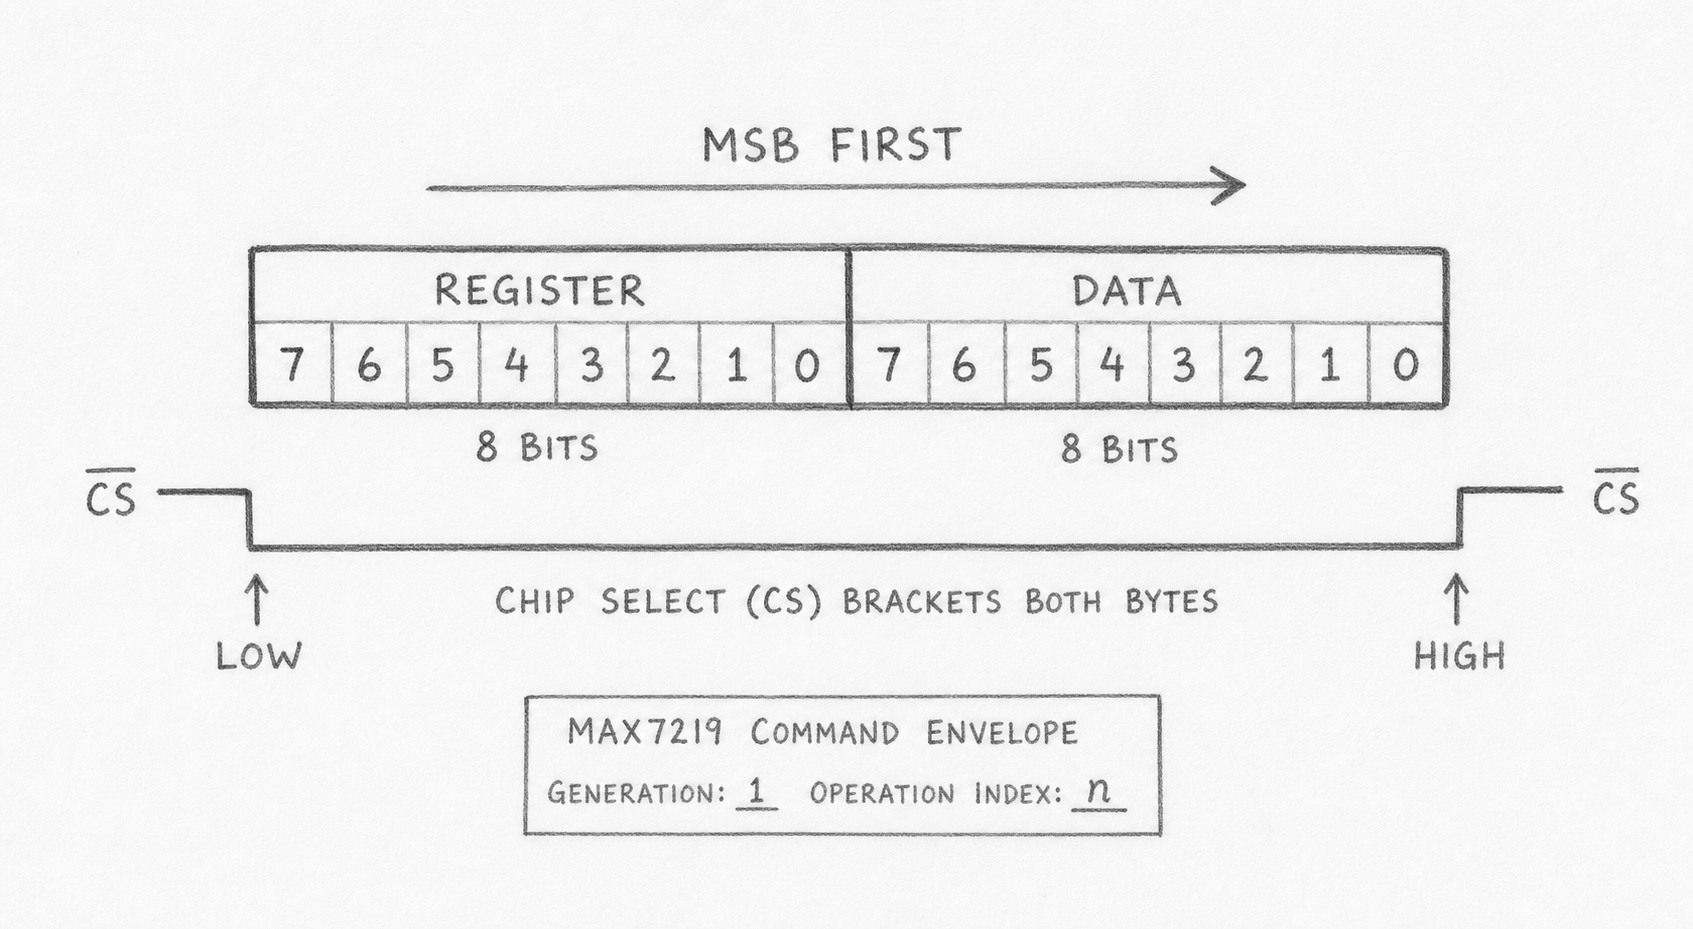
\includegraphics[width=0.96\linewidth,height=1.95in,keepaspectratio]
 {059-register-envelope-pencil.png}

\small\textit{Alternative text: a pencil-drawn envelope contains correlation
fields beside two ordered byte cards, first register address and then data,
with an MSB-first arrow and a chip-select bracket around both bytes.}
\end{center}

\begin{tabularx}{\linewidth}{@{}l l X@{}}
\toprule
Register intent & Address & E0 meaning\\
\midrule
decode mode & \texttt{0x09} & request no BCD decoding\\
intensity & \texttt{0x0A} & request a validated value from 0 through 15\\
scan limit & \texttt{0x0B} & request all eight rows\\
shutdown & \texttt{0x0C} & request dark or normal operation\\
display test & \texttt{0x0F} & request test off\\
row 1 through 8 & \texttt{0x01}--\texttt{0x08} & request transformed row data\\
\bottomrule
\end{tabularx}

The canonical replay fixes intensity at 1. That is a logical register value,
not proof of safe LED current. A future powered adapter must qualify the exact
module, RSET network, supply, current, and thermal behavior.

\section{Let the caller pace transport}
The policy never invokes SPI code. One service call may publish at most one
command. The caller records the two-byte transaction and later returns one
copied receipt. That split keeps policy replay deterministic and prevents a
hidden retry, wait, callback, or catch-up loop.

\begin{center}
% ADK visual: pencil
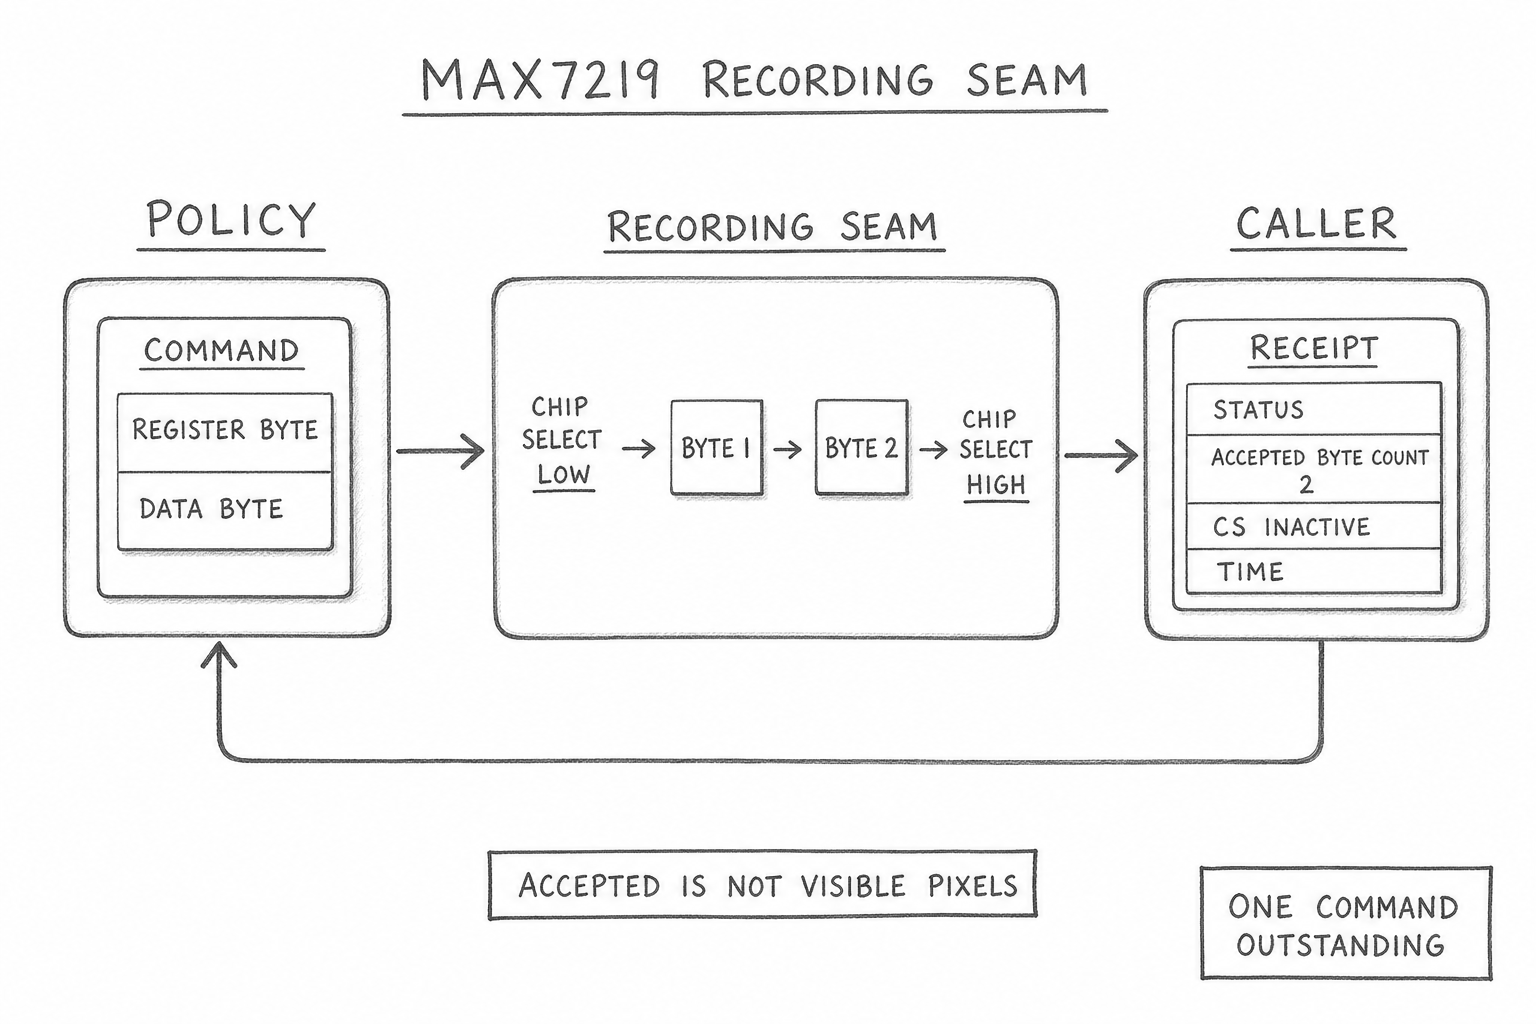
\includegraphics[width=0.95\linewidth,height=2.10in,keepaspectratio]
 {059-recording-seam-pencil.png}

\small\textit{Alternative text: a hand-drawn policy box passes one command
card to a recording transport box; a separate receipt card returns with the
same correlation fields, byte count, chip-select cleanup mark, time, and
status.}
\end{center}

A successful receipt requires all three facts:
\begin{itemize}
 \item \texttt{Status::Ok};
 \item exactly two accepted bytes; and
 \item chip select recorded inactive afterward.
\end{itemize}
No single fact substitutes for the others. A non-OK receipt may report zero or
one accepted byte. Non-OK with two accepted bytes, or OK with a short byte
count, is contradictory evidence and faults without advancing the generation.

\begin{tabularx}{\linewidth}{@{}l c c X@{}}
\toprule
Status & Accepted bytes & CS inactive & Disposition\\
\midrule
OK & 2 & yes & accept the outstanding command\\
OK & 0 or 1 & either & contradictory; fault\\
non-OK & 0 or 1 & yes & transport failure with exact prefix\\
non-OK & 2 & either & contradictory; fault\\
either & any & no & cleanup evidence failed\\
\bottomrule
\end{tabularx}

\section{Correlate before mutating}
A receipt belongs to exactly one outstanding command. Its owner, lifecycle,
configuration, presentation generation, operation index, register, and data
must match. Observation time must be valid under modular ordering. An exact
duplicate is idempotent; a changed duplicate, foreign receipt, stale receipt,
regression, or exact-half-range timestamp rejects atomically.

\begin{lstlisting}
command = policy.service(noReceipt);
recorded = transport.record(command);
receipt = copyReceipt(command, recorded);
result = policy.service(receipt);
\end{lstlisting}

This pseudocode names the evidence flow; the canonical sketch contains the
exact API. Before running it, predict which state may change after each line:
\begin{itemize}[leftmargin=1.4em]
 \item \textbf{Command published:} one command is outstanding; no receipt has
       been accepted.
 \item \textbf{Transport recorded:} the policy is unchanged; the caller owns
       the copied trace.
 \item \textbf{Matching receipt accepted:} the operation may advance by
       exactly one.
 \item \textbf{Foreign receipt supplied:} no accepted state changes.
\end{itemize}

\section{Make partial writes impossible to forget}
A MAX7219 update is not physically atomic. If the first byte was accepted and
the second failed, the controller cannot roll the display back. The policy
therefore preserves desired state, last fully submitted state, accepted
partial prefix, blank request, cleanup state, and physical indeterminacy as
different facts.

\begin{center}
% ADK visual: pencil
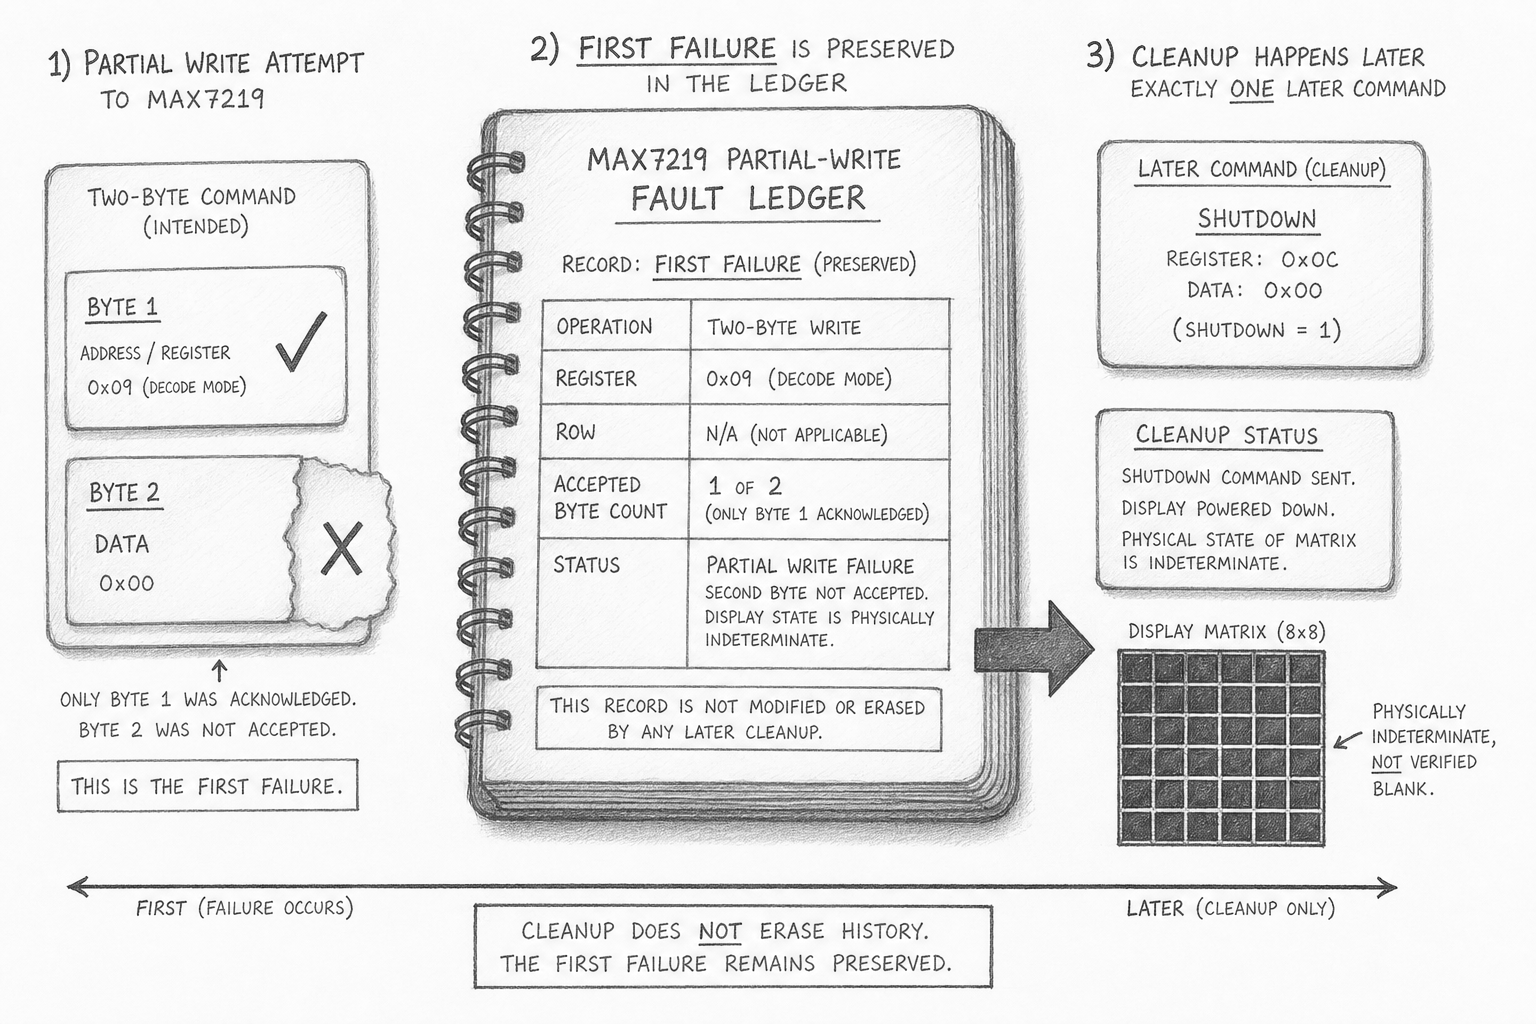
\includegraphics[width=0.96\linewidth,height=2.15in,keepaspectratio]
 {059-fault-ledger-pencil.png}

\small\textit{Alternative text: a pencil incident ledger preserves the first
failed operation, register, row, accepted-byte count, and status; a later
one-command shutdown attempt is recorded in a separate cleanup box and never
erases the primary entry.}
\end{center}

After a failure, cleanup is pending. A later service call may request exactly
one best-effort shutdown command. Its result is secondary evidence: cleanup
status never overwrites the primary fault provenance. Even an accepted
shutdown command proves only that the recording seam accepted its bytes. It
does not prove that a physical matrix went dark.

\lessonbox{\textbf{Fault rule.}
Preserve the first failure. Bound cleanup to a later single command. Label the
physical presentation indeterminate until an electrically qualified endpoint
provides stronger evidence.}

\section{Commit a complete frame, then submit rows}
Frame candidates use the same transaction vocabulary as Lesson 058:
\texttt{preview()}, \texttt{canCommit()}, and \texttt{commit()}. A preview is
bound to owner, lifecycle, configuration, and base generation. Commit copies a
complete desired frame but issues no transport command. Submitted generation
advances only after all eight row receipts are accepted.

\begin{tabularx}{\linewidth}{@{}l X X@{}}
\toprule
State & What it proves & What it does not prove\\
\midrule
desired & a complete frame was committed locally & any command was accepted\\
partial prefix & some command prefix was accepted & a complete register write\\
last fully submitted & all eight row receipts passed & visible pixels or atomic update\\
shutdown accepted & shutdown bytes passed the seam & optical blanking\\
physically indeterminate & evidence cannot establish endpoint state & that the endpoint is lit or dark\\
\bottomrule
\end{tabularx}

The later Lesson 060 coordinator can preflight both display policies before
either pure commit. That produces one coherent logical snapshot, not
simultaneous photons.

\section{Run the canonical replay}
Open
\texttt{examples/Lesson059Max7219Presentation/}\\
\texttt{Lesson059Max7219Presentation.ino}. Follow its narrative order:
\textbf{acquire} the recording cells, \textbf{configure} orientation and
intensity, \textbf{start} dark, then repeatedly
\textbf{observe}, \textbf{decide}, and \textbf{present} one copied command.

Before running, record three predictions:
\begin{enumerate}
 \item The first configuration register is \blankline.
 \item Normal operation is requested before/after row clearing: \blankline.
 \item A row-4 second-byte failure records accepted-byte count \blankline.
\end{enumerate}

After running, inspect the named non-Serial result cells. Serial output may
explain the trace, but it is not the only proof.

\begin{tabularx}{\linewidth}{@{}X X X@{}}
\toprule
Observation cell & Expected result & Interpretation\\
\midrule
configuration-order result & exact golden order accepted & policy starts dark and enables last\\
orientation result & asymmetric frame matches expected rows & transform is explicit\\
fault-provenance result & first failure and cleanup remain separate & no invented rollback\\
shutdown result & copied shutdown receipt recorded & logical request only\\
\bottomrule
\end{tabularx}

\section{Diagnose evidence, not imagined hardware}
\begin{tabularx}{\linewidth}{@{}X X X@{}}
\toprule
Observed evidence & Likely policy meaning & Next check\\
\midrule
no command emitted & receipt still outstanding or lifecycle inactive &
inspect outstanding identity and lifecycle\\
receipt rejected without mutation & correlation, time, or structure mismatch &
compare every copied field\\
cleanup pending & primary command failed or evidence contradicted itself &
inspect first failure before cleanup\\
submitted generation unchanged & fewer than eight row receipts accepted &
find the first incomplete row operation\\
orientation mismatch & transform expectation differs from configuration &
replay one asymmetric pixel\\
\bottomrule
\end{tabularx}

\section{Know the E0 boundary}
This lesson proves deterministic frame transformation, exact register intent,
one-command service, receipt correlation, partial-prefix provenance, bounded
cleanup, lifecycle behavior, and compile-only Mega integration. It does not
prove SPI electrical timing, module identity, RSET value, decoupling, matrix
orientation, current, startup state, visible presentation, or safe blanking.

Before E1b promotion, record:
\begin{itemize}
 \item exact MAX7219 IC or module revision and authoritative schematic;
 \item matrix anode/column and cathode/row mapping plus observed orientation;
 \item RSET and decoupling values, supply compatibility, and logic levels;
 \item serial timing, loaded-rail current, startup, fault, and shutdown evidence;
 \item a central resolution for the existing \texttt{SpiBus} terminal-fault
 recovery ambiguity before any MAX7219 adapter is added.
\end{itemize}
An unknown or low-value current-setting resistor may exceed the project's
100 mA USB campaign. Keep the module unpowered until its exact network is
qualified.

\section{Exit ticket}
\begin{enumerate}
 \item Why is a successful two-byte recording receipt not pixel evidence?
 \item Why must an identical duplicate be idempotent but a changed duplicate
 reject?
 \item Which state advances only after all eight row receipts pass?
 \item Why is cleanup scheduled for a later service call?
 \item Name two physical facts required before E1b promotion.
\end{enumerate}

\lessonbox{\textbf{Completion evidence.}
You can predict the initialization order, transform an asymmetric frame,
trace one command and matching receipt, explain every contradictory receipt,
and distinguish a fully submitted logical frame from visible hardware state.
Bench acceptance remains explicitly deferred.}

\vfill
\footnotesize
\textbf{Canonical companions:}
\href{https://github.com/spincyc/adk/blob/main/examples/Lesson059Max7219Presentation/Lesson059Max7219Presentation.ino}{Lesson 059 sketch}
\quad
\href{https://github.com/spincyc/adk/blob/main/site/pages/lessons/059.md}{HTML lesson source}
\quad
\href{https://github.com/spincyc/adk/blob/main/docs/design/LESSONS_058_060_DISPLAY_TIMING_DESK_PLAN.md}{implementation plan}
\end{document}
